%%====================================================================%%
%%                	AGH University of Science and Technology
%%	Faculty of Electrical Engineering, Automatics, IT and Electronics
%%			Department of Computer Science
%%				Master's thesis
%%
%%            Author : Adrian Wolny
%%        Speciality : Distributed systems and computer networks
%%      Register No. : 203789
%% Thesis Supervisor : Prof. dr hab. in�. Robert Schaefer
%%    Date (version) : 01.06.2011 0.1
%%
%%--------------------------------------------------------------------%%

\documentclass[pdflatex,11pt]{aghdpl}
%%\usepackage[polish]{babel}
\usepackage[utf8]{inputenc}
\usepackage{amsthm}
\usepackage{enumerate}
%%\usepackage{minted}
\usepackage{array}
\usepackage{algorithm}
\usepackage{algorithmic}
\usepackage{amsmath}
\usepackage{amsfonts}
\usepackage{listings}

\graphicspath{{./img/}}


\renewcommand{\topfraction}{0.85}
\renewcommand{\textfraction}{0.1}

\newtheorem{definition}{Definition}
%%\newtheorem{przyklad}{Przyk�ad}

%%\newminted{java}{gobble=4, linenos, numbersep=8pt}
%%\newminted{js}{gobble=4, linenos, numbersep=8pt}
%%\newminted{xml}{gobble=4, linenos, numbersep=8pt}
%%\renewcommand{\theFancyVerbLine}{\ttfamily\small\oldstylenums{\arabic{FancyVerbLine}}}

%---------------------------------------------------------------------------

\author{Adrian Wolny}

%%\titlePL{Poprawa algoryt�w populacyjnych w problemach optymalizacji globalnej
%%poprzez deterioracj� funkcji przystosowania}
\titleEN{Improving population-based algorithms used in Global Optimization with
Fitness Deterioration techniques}

%%\thesistypePL{Praca magisterska}
\thesistypeEN{Master of Science Thesis}

%%\supervisorPL{Prof. dr hab. in�. Robert Schaefer}
\supervisorEN{Robert Schaefer, Prof., PhD, DSc}

\date{2011}

%%\departmentPL{Katedra Informatyki}
\departmentEN{Department of Computer Science}

%%\facultyPL{Wydzia� Elektrotechniki, Automatyki, Informatyki i Elektroniki}
\facultyEN{Faculty of Electrical Engineering, Automatics, Computer Science and Electronics}

\acknowledgements{I would like to thank Prof. Schaefer 
for his invaluable support and motivation throughout the duration of my work}

\setlength{\cftsecnumwidth}{10mm}

%---------------------------------------------------------------------------

\begin{document}

\titlepages

\tableofcontents

\clearpage


\chapter{Introduction}
\label{Introduction} 

\begin{quotation}
 It is impossible for any optimization algorithm to outperform random walks on all possible problems.
\end{quotation}
\begin{flushright}
 ... a conclusion from No Free Lunch Theorem
\end{flushright}

\section{A statement of a problem}

A Global Optimization Algorithm is defined as optimization algorithm
that employs measures that prevent convergence to local optima
and increase the probability of finding a global optimum. 

Evolutionary algorithms are known as a generic population-based metaheuristics
which often perform well approximating solutions to all
types of problems because they ideally do not make any assumption about the underlying fitness landscape; 
this generality is shown to be a great successes in many real-life problems. 
Evolutionary algorithms have the tendency to lose diversity within their
population of feasible solutions and to converge into a single solution.
However, there are domains where the global solution may not suffice. 
Such problems require the location and maintenance of multiple robust local
solutions, i.e local solutions whose basins of attraction areproperly wide and deep.

The most common technique in evolutionary algorithm which is
used to achieve this goal is to incorporate some sort of niching method
like crowding or fitness sharing which promote diversity of population,
which in turn delay premature convergence and likely enable the algorithm to
find multiple optimal solutions in single population.
 
Standard niching methods are often inefective and hard to introduce 
in existing evolutionary algorithms. In this paper we adopt a
different approach to multimodal function optimization. Instead of
embedding a niching method in the evolutionary algorithm itself we
use a hybrid approach in which we perform several runs of a evolutionary 
algorithm and alter the fitness function in every subsequent
run in a way that prevents exploration of basins of attraction which
were found in previous runs of the algorithm.

In each iteration we run EA, then cluster received population and
based on the assumption that clusters of individuals obtained from
the clustering algorithm are located in basins of attraction we interpolate
 each basin by multidimensional Gaussian function. By combining
these functions with current objective function in a proper way we
create deteriorated fitness function which will discourages future runs
from revisiting the same area.

This work tries to find an effective fitness deterioration technique in
high-dimensional domain spaces. We have implemented a general-purpose framework which can be
used to test our fitness deterioration techniques in conjunction with
various evolutionary algorithms. While our algorithm may be used with many types
of EAs it would be the most efficient when used with algorithms which are capable 
of finding many local solutions in single run. This is why for tests
we choose so called Hierarchical Genetic Strategy which performs efficient
concurrent search in the optimization landscape by many small populations.

The quality of the deterioration process strongly depends on clustering results.
We choose density-based algorithm called OPTICS as with this method we can extract clusters of
different densities very efficiently and choose clusters which give the
best accuracy of fitness deterioration process.

\section{Related Work}

As mentioned before this work focus on finding solutions for multi-modal
optimization tasks. There are many publications which decsribes how to extend
EAs to multi-modal optimization. Most of them focuses on 
\textit{Niching methods} \cite{niching,sharing,dynsharing} which address this
issue by maintaining a population of diverse solutions througout the time and this way they allow
parallel convergence into multiple good solutions in multimodal domains.

Our solution works by iterating a simple GA and maintaining the best solution of
each run off-line, by detection of basins of attraction and degeneration of
fitness landscape. We may consider our algorihtm as a variant of
\textit{Sequential niching} approach (throughout this paper we use terms 
\textit{Sequential niching} and \textit{Fitness deterioration} interchangeably).

At this point it is worth mentioning some of the works of Prof. A. Obuchowicz 
especially the publication \cite{esss} which is the only one I found which 
use the term \textit{fitness deterioration} explicitly.
In \cite{esss} he describes ESSS-DOF algorithm (Evolutionary Search with Soft
Selection with Deterioration of Objective Function) as an extension to the ESSS
method which maintaing population diversity by the following schema:
\begin{quotation}
When the population converges to local optimum we degenerate the objective 
function which cause the rapid migration of individuals and enable the 
population to escape for the local optimum.
\end{quotation}

The algorithm degenerate the objective function by composing it with Gaussian
function which approximate the local optimum. Our deterioration algorithm
described in detail in chapter 4 uses Gaussian functions as well
(Gaussian function has got many useful properties which makes it well-suited
to the fitness deterioration. We describe these characteristics in chapter 4).

Mentined methods are incorporated directly into the basic cycle of evolutionary
algorithm which differs from our \textit{Sequential niching} technique. 
The sequential niching approach has several advantages:

\begin{itemize}
  \item it is simple to incorporate in existing optimization methods
  \item it efficiently finds many local solutions
  \item it provides reasonable stop criterion which in this case is based on the
  quality of clusters returned by the clustering algorithm
\end{itemize}





\chapter{Algorithm}
\label{Algorithm}

\section{A Hybrid Approach}

Our deterioration algorithm may be easily incorporated in existing optimization
methods. This can be expressed as a general hybrid approach to global
optimization in which we do not change the implementation of the used EA
but treat it as an integral element of our iterative process.
This can be visualized by the following pseudo code:




\begin{algorithmic}[1]
\WHILE{$i < getIterationCount()$}
	\STATE {$execute(evolutionaryAlgorithm)$}
	\STATE {$population=getPopulation(evolutionaryAlgorithm)$}
	\STATE {$clusters=cluster(population)$}
	\IF{$clusters.isEmpty()$}
		\STATE {$break$}
	\ENDIF
	\STATE {$detFitness=performCrunching(clusters,currentFitness)$}
	\STATE {$saveClusters(clusters)$}
	\STATE {$updateFitness(detFitness)$}
\ENDWHILE
\STATE {$execute(evolutionaryAlgorithm)$}
\STATE {$extractBestClusters()$}
\end{algorithmic}




The condition in while statement should be treated as control statement rather
than the real termination criterion. It may be useful in cases where the
clustering algorithm is misconfigured and always returns some clusters in which
case the condition would prevent our algorithm to run endlessly.
Our actual stop criterion is based on the condition inside the loop (line 5): if the clustering algorithm did not find any group of similar individuals or the group has low quality measures it jumps out
of the loop and then we perform the last invocation of the EA in order to
increase the probability of finding the local optimum which has not been explored during iterations.

Using this general scheme has one important advantage: we do not have to change
existing implementation of a given EA in contrast to standard niching
methods which must be incorporated directly in the evolutionary algorithm. But
what is more important, it provides a reasonable stop criterion which in this case is based 
on the quality of clusters returned by the clustering algorithm.
 
In the subsequent chapters we will describe components  of the general
algorithm in more details.
In chapter 3 we will discuss the clustering method used in our algorithm and 
how does it influence the deterioration process. Chapter 4 describes
deterioration algorithm in more detail and chapter 5 shows the results 
of the tests.




\chapter{Clustering}
\label{Clustering}

Clustering algorithms divide a dataset into several disjoint subsets. All elements in such
a subset share common features like, for example, spatial proximity.
Clustering is used as a stand-alone tool to get insight into the distribution
of a data set or as a preprocessing step for other algorithms operating on the
detected clusters. The former can be used to determine stop
criteria (see section 3.2) and the latter is used in our deterioration
schema (see chapter 4).

\section{Cluster Extension}

Basin of attraction is a term used in dynamic systems
defined as the set of initial conditions leading to long-time 
behavior that approaches the particular attractor.
In the field of global optimization, basin of attraction may
be defined in the following way.

\begin{definition}\label{def:basin}
\textbf{Basin of attraction} is a subset A of the problem space which contains
local solution and for each point which belongs to A the gradient of the objective
function at that point will lead towards the solution.
\end{definition}

Clusters may be seen as an approximation of the basin of attraction, because
the distribution of individuals which flooded to the basins
provides useful information about its size and shape. So the clustering 
algorithm may be used to detect the set of individuals which belongs
to the same basin of attraction. Such a set may be later described by extracting
some statistical information from that set, e.g the center point,  
the radius of the set, covariance matrix etc. This is what we called
a \textbf{Cluster extension}. 
Not only does our algorithm efficiently solve multimodal problems, it also
provides information about detected sets (basins of attraction) in the from 
of cluster extensions. 

\section{Clustering as a Stop Criterion}

The termination criterion in classic evolutionary algorithms is hard to define
and very often problem dependent, as we do not have any global information about 
the fitness landscape and therefore we can only compare one solution to another
previously found. 
Some of the common termination criteria such as: 
\begin{itemize}
  \item maximum computation time
  \item total number of iterations
  \item no improvement for a specified number of iterations
\end{itemize}
are only applicable to a specific problems and none of them can be used
as a general stop criterion. 
The clustering, which is performed in every iteration, 
on the other hand may give us some clues about the global
characteristics of the fitness landscape i.e. when the clustering algorithm performed 
on the final population finds nothing it is very likely that in previous
iterations we have deteriorated the fitness landscape in places where 
the most desirable solutions reside and there is no use in continuing the
searching process. This is considered to be true because we are looking for
robust solutions which are resistant to noise and lie in basins of attraction 
which are significantly wide and deep. The population of EA is likely 
to converge to such solutions, so having found no clusters of individuals after
performing the EA in a given iteration shows that the population does not converge 
to any robust solution. In such circumstances we terminate the main loop
of the algorithm.

\section{OPTICS}

We have choosen density-base clustering algorihtm called \textit{OPTICS:
Ordering Points To Identify the Clustering Structure} \cite{optics}. In density
clustering clusters are regarded as regions in the data space in which the objects are 
dense and which are separated by regions of low object density. These regions
may have an arbitrary shape and the points inside a region may be arbitrarily
distributed.

\textit{OPTICS} is an extendsion to a well-known density clustering algorithm
called \textit{DBSCAN}. The basic idea for \textit{DBSCAN} is that for each
point of a cluster the neighborhood of a given radius $\epsilon$ has to contain
at least a minimum number of points $minPts$.

\textit{OPTICS} works like \textit{DBSCAN} but for an infinite number of
distance paramters $\epsilon_i$ which are smaller than a \textit{generating distance}
$\epsilon$. The only difference is that we do not assing cluster memberships.
Instead, we store the \textbf{order} in which the objects are processed (the
main priniple is that we always have to select an object which is
density-reachable with respect to the lowest $\epsilon$ value to guarantee that
clusters with higher density are finished first) and the information which would
be used by \textit{DBSCAN} algorithm to assing cluster memberships. This
information consists of only two values for each object: \textit{core-distance}
and \textit{reachability-distance}.


\begin{definition}\label{def:core-distance} 
\textbf{core-distance} - the core-distance of an object $p$
is simply the smallest distance $\epsilon'$ between $p$ and an object in its
$\epsilon$-neighborhood such that $p$ would be a core object with respect to
$\epsilon'$ if this neighbor is contained in $N_\epsilon(p)$. Otherwise, the
core-distance is \textit{UNDEFINED}
\end{definition}


\begin{definition}\label{def:reachability-distance} 
\textbf{reachability-distance} - the reachability-distance
of an object $p$ with respect to another object $o$ is the smallest distance such that $p$ is
directly density-reachable from $o$ if $o$ is a core object
\end{definition}

This information is sufficient to extract all density-based clusterings
with respect to any distance $\epsilon'$ which is smaller that the generating
distance $\epsilon$

An advantage of cluster-ordering a data set compared to other clustering methods
is that the ordering which might be visualized by \textit{reachability-plot} of
ordered points is rather insensitive to the input parameters of the method i.e.
the \textit{generating distance} $\epsilon$ and the value for $minPts$. Roughly
speaking, the values have just to be \textit{large} enough to yield a good
result. The concrete values are not crucial because there is a broad range of
possible values for which we always can see the clustering structure of a data
set when looking at the corresponding \textit{reachability-plot}. Figure 3.1
shows the result of \textit{OPTICS} clustering for a sample set of points.
Figure 3.2 shows reachablity plot for various \textit{generating distances} -
$\epsilon$. 

The next chapter describes how \textit{OPTICS ordering} properties are used
to prevent degradation of areas which have not been explored during the course
of the algorithm. 

\begin{figure}
  \centering
  \fbox{
    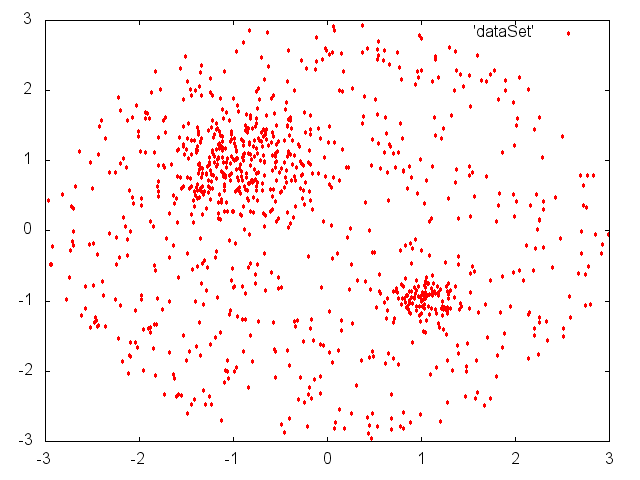
\includegraphics[scale=0.4]{dataSet.png}
  }
  \fbox{
    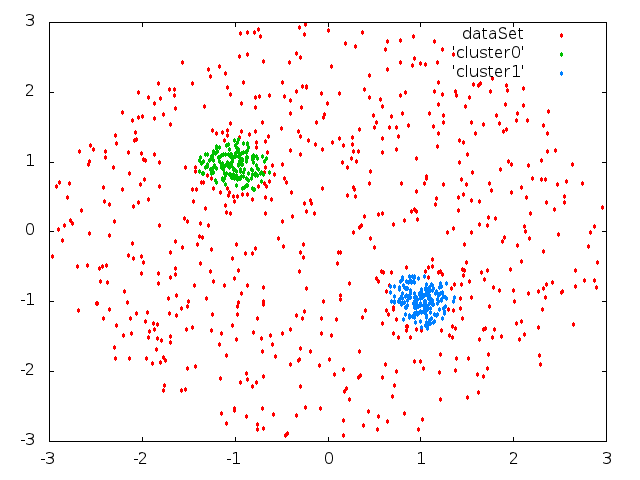
\includegraphics[scale=0.4]{clusters.png}
  }
  \caption{Visualization of the DBSCAN algorithm applied to Optics ordering
  of simple 2-dimensional data set which consists of 1000 points. Optics
  paramters: $minPts=20, \epsilon=1.2$, the two clusters was found using DBSCAN
  paramters: $\epsilon'=0.2$ }
  \label{clusters}
\end{figure}


\begin{figure}
  \centering
  \fbox{
    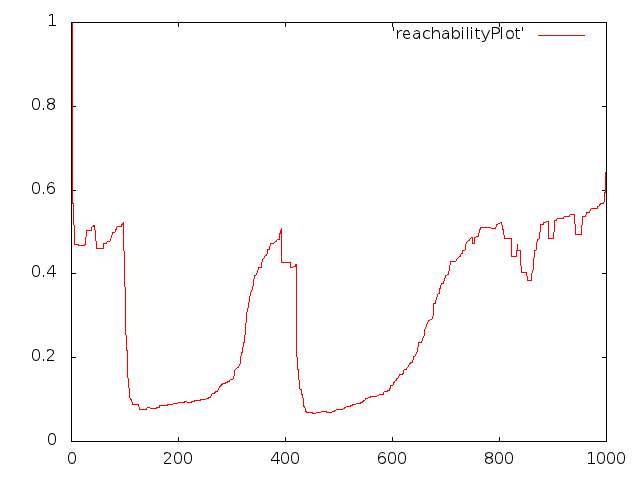
\includegraphics[scale=0.4]{reachability1/1_5_20.png}
  }
  \fbox{
    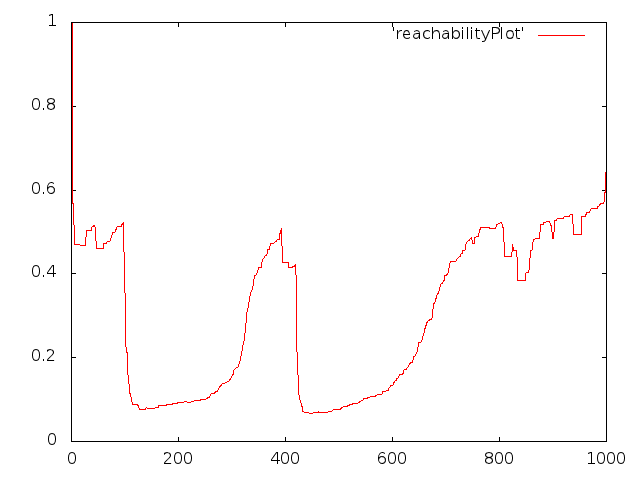
\includegraphics[scale=0.4]{reachability1/1_0_20.png}
  }
  \fbox{
    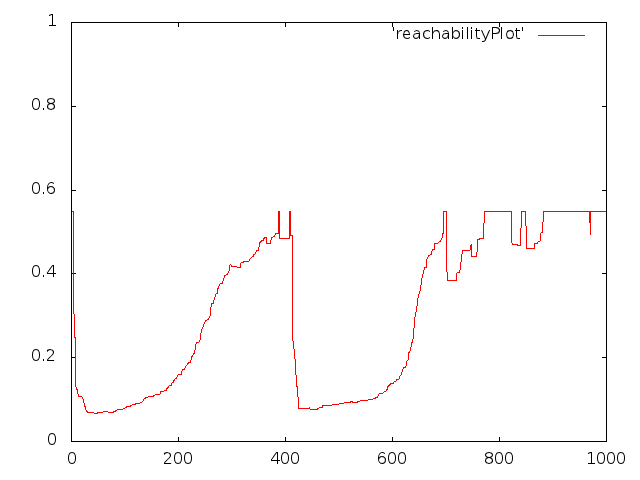
\includegraphics[scale=0.4]{reachability1/0_5_20.png}
  }
  \caption{Reachability plot for data set presented on figure 3.1. Optics
  paramters (minPts, $\epsilon$) are: (20, 1.5), (20, 1.0), (20, 0.5)
  respectively. The two cavities which are visible in each plot depict the two
  of the clusters on figure 3.1. This proves that there is a large range of
  values for $\epsilon$ (\textit{generating distance}) for which the appearance
  of the reachability plot will not change significantly. (the flat shape of function from the last plot
  results from the fact that we truncate the reachability-distance to the 
  generating distance $\epsilon$, when the former is greater than the latter)}
  \label{reach}
\end{figure}



\chapter{Fitness Deterioration}
\label{ch:fitnessDet}

This chapter contains detailed description of the deterioration algorithm
which is the central point of the \textit{Cluster Supported Fitness
Deterioration} algorithm described in chapter \ref{ch:csfdAlgorithm}. 
Before diving into the details, here is the formal definition of the fitness
deterioration process:
\textit{Fitness Deterioration} is a process of degrading the fitness
function in areas occupied by groups of individuals obtained from
clustering (see Section \ref{sec:Fdt} and references inside). 
We suggest to achieve this goal in the CSFD strategy by creating a linear combination 
of the current fitness function and \textit{crunching functions} which approximate
the fitness in subsets of problem domain occupied by clusters.
Let $F_k$ be the fitness function in $k$-th iteration of CSFD
(i.e. in the $k$-th execution of the main loop of the Algorithm \ref{alg:CSFD})
and $C_1, \ldots, C_{M_k}$ be
$M_k$ clusters found in $k$-th iteration of our new sequential niching algorithm 
(algorithm \ref{alg:CSFD} described in Section \ref{sec:algDesc}).
For each cluster $C_i$ we create the \textit{crunching function} $g_i$ and then
we construct deteriorated fitness $F_{k+1}$ (which will be used in the
$(k+1)$-th iteration) as follows:

\begin{equation}
\label{eqn:fitDet}
F_{k+1} = F_k + \sum_{i=1}^{M_k} \alpha_i g_i,
\end{equation}
where the selection of the functional coefficients 
$\alpha_1, \ldots, \alpha_{M_k}; \; \alpha_i:\mathcal{D} \rightarrow \mathbb{R}_+, \,
i = 1, \ldots, M_k$ depends on the
type of deterioration used and will be described later in Sections
\ref{sec:BasScheme}, \ref{sec:WeightScheme}
(see formulas (\ref{eqn:alpha1}), (\ref{eqn:alpha2}), 
(\ref{eqn:fractures})).
 

The \textit{Crunching function} $g_i: \mathcal{D} \rightarrow \mathbb{R}_+$ 
is constructed for each newly recognized cluster of individuals
$C_i \subset P$.
Based on the assumption that clusters lie inside basins
of attraction and that the distribution of individuals inside the cluster
is a good approximation of the shape of the basin occupied by the cluster,
the deterioration algorithm tries to exploit information
provided by the clustering algorithm and based 
on that information it augments the fitness function in order to minimize 
the probability of finding already explored basins of attraction in further iterations.

We may ask ourselves why we do not prevent exploration of basins 
we found in previous iterations simply by remembering the regions occupied
by clusters and ignoring individuals which fall in this regions.
The answer is probably the most important reason why we have chosen fitness
deterioration for this task. 
We can not prevent individuals to explore
neighborhood of solutions found in previous iterations because such
approach would cause our meta-heuristic to loose \textit{completeness} (see
\cite{PardalosRomeijn2002}).

\begin{definition}\label{completeness}
A set $Op$ of search operations searchOp is \textit{complete}
if and only if every point $g_1$ in the search space \mathbb{G}
can be reached from every other point $g_2 \in \mathbb{G}$ by applying
only operations $searchOp \in Op$.
\begin{equation}
\forall g_1, g_2 \in \mathbb{G} \Rightarrow \exists k \in \mathbb{N}:
P(g_1=Op^k(g_2)) > 0
\end{equation} 
\end{definition}

If the set of search operations is not complete, there are points 
in the search space which cannot be reached. 
Then, we are probably not able to explore the problem space adequately 
and possibly will not find satisfyingly good solution. 
That is why it is better to use fitness deterioration as a way to discourage
rather then prevent individuals from sinking to the same basins of attraction twice.

Here we would like to emphasize the fact that the
deterioration process does not try to accurately interpolate the fitness
function in the neighborhood of the solution because it would be very
expensive in a high dimensional spaces. Instead it tries to find simple
crunching functions which would sufficiently degrade the fitness landscape in the areas 
occupied by the clusters and then remove the individuals from these regions
in the next CSFD steps with the sufficiently high (but even less then 1) probability.


We now can define what are the characteristics of a good deterioration
algorithm:
\begin{itemize}
  \item \textit{It has to be chep} in terms of space and time. We are looking
  for methods which can be successfully applied for solving high
  dimensional functions' optimization. After every iteration the resulting
  fitness function is the linear combination of crunching functions, therefor we
  must ensure that computation of a single crunching function is $O(1)$ and does 
  not depend no the number of individuals inside a cluster or the number of
  clusters. Resulting fitness must be $O(k)$ where $k$ is the number of
  solutions (clusters) found in previous iterations.
  
  \item \textit{It has to discourage the population of EA from visiting the
  neighborhood of solutions found in previous iterations twice}. We do not want
  these regions to be inaccessible as this would break the \textbf{completeness} 
  of our algorithm, we just want an individual to be given a low fitness when it
  finds itself in these regions.
  
  \item \textit{It has to be easy to extend for subsequent solutions}. The way
  we construct fitness function in subsequent iterations already fulfills
  this requirement. To extend the deterioration for subsequent solutions we
  simply add new crunching functions multiplied by the scaling factors we define
  later in this chapter. 
\end{itemize}


\begin{definition}\label{premature-convergence}
\textit{Premature Convergence} \cite{PardalosRomeijn2002} An optimization process has
\textit{prematurely converged} to a local optimum if it is no longer able to explore 
other parts of the search space than the area currently being examined and there 
exists another region that contains a superior solution.
\end{definition}

The premature convergence is not a problem in our algorithm, because once the
population finds itself in the local optima trap it is very likely that the
population will be avoiding this region in the next iterations. Actually we
encourage an optimization process performed by the used EA (e.g. SGA) 
to converge quickly to local solution in order to find new solutions 
faster in the next iterations. 

An ideal GA engine to be used in our hybrid algorithm defined in Section
\ref{sec:algDesc} would be the one which produces many small populations in problem space and
each population would use strong selection pressure with small mutation rate
with high recombination rate to increase exploitation. This is why Hierarchical 
Genetical Search (HGS) \cite{WierzbaSemczukKolodziejSchaefer2003} algorithm
would be perfect for our needs as it possess all of the listed characteristics. 
However we may also choose some simple 
SGA or Evolution Strategy with small population size and strong exploitation
characteristics.
 

\section{Fitness deterioration and clustering}
\label{sec:FitDetClust}

To increase the accuracy of the fitness deterioration process 
we want to use the maximum amount of information provided by the clustering
algorithm. As we mentioned at the begining of this chapter we create one
crunching function per cluster which, depending on the shape of the cluster, 
may not be very accurate or may even degrade areas
of the fitness landscape which have not been explored yet and potentially
contain valuable solutions. 
Figure \ref{fig:hardClusters1} shows cases in which
crunching functions created for extracted clusters strongly affect regions outside the clusters.

\begin{figure}
  \centering
  \fbox{
    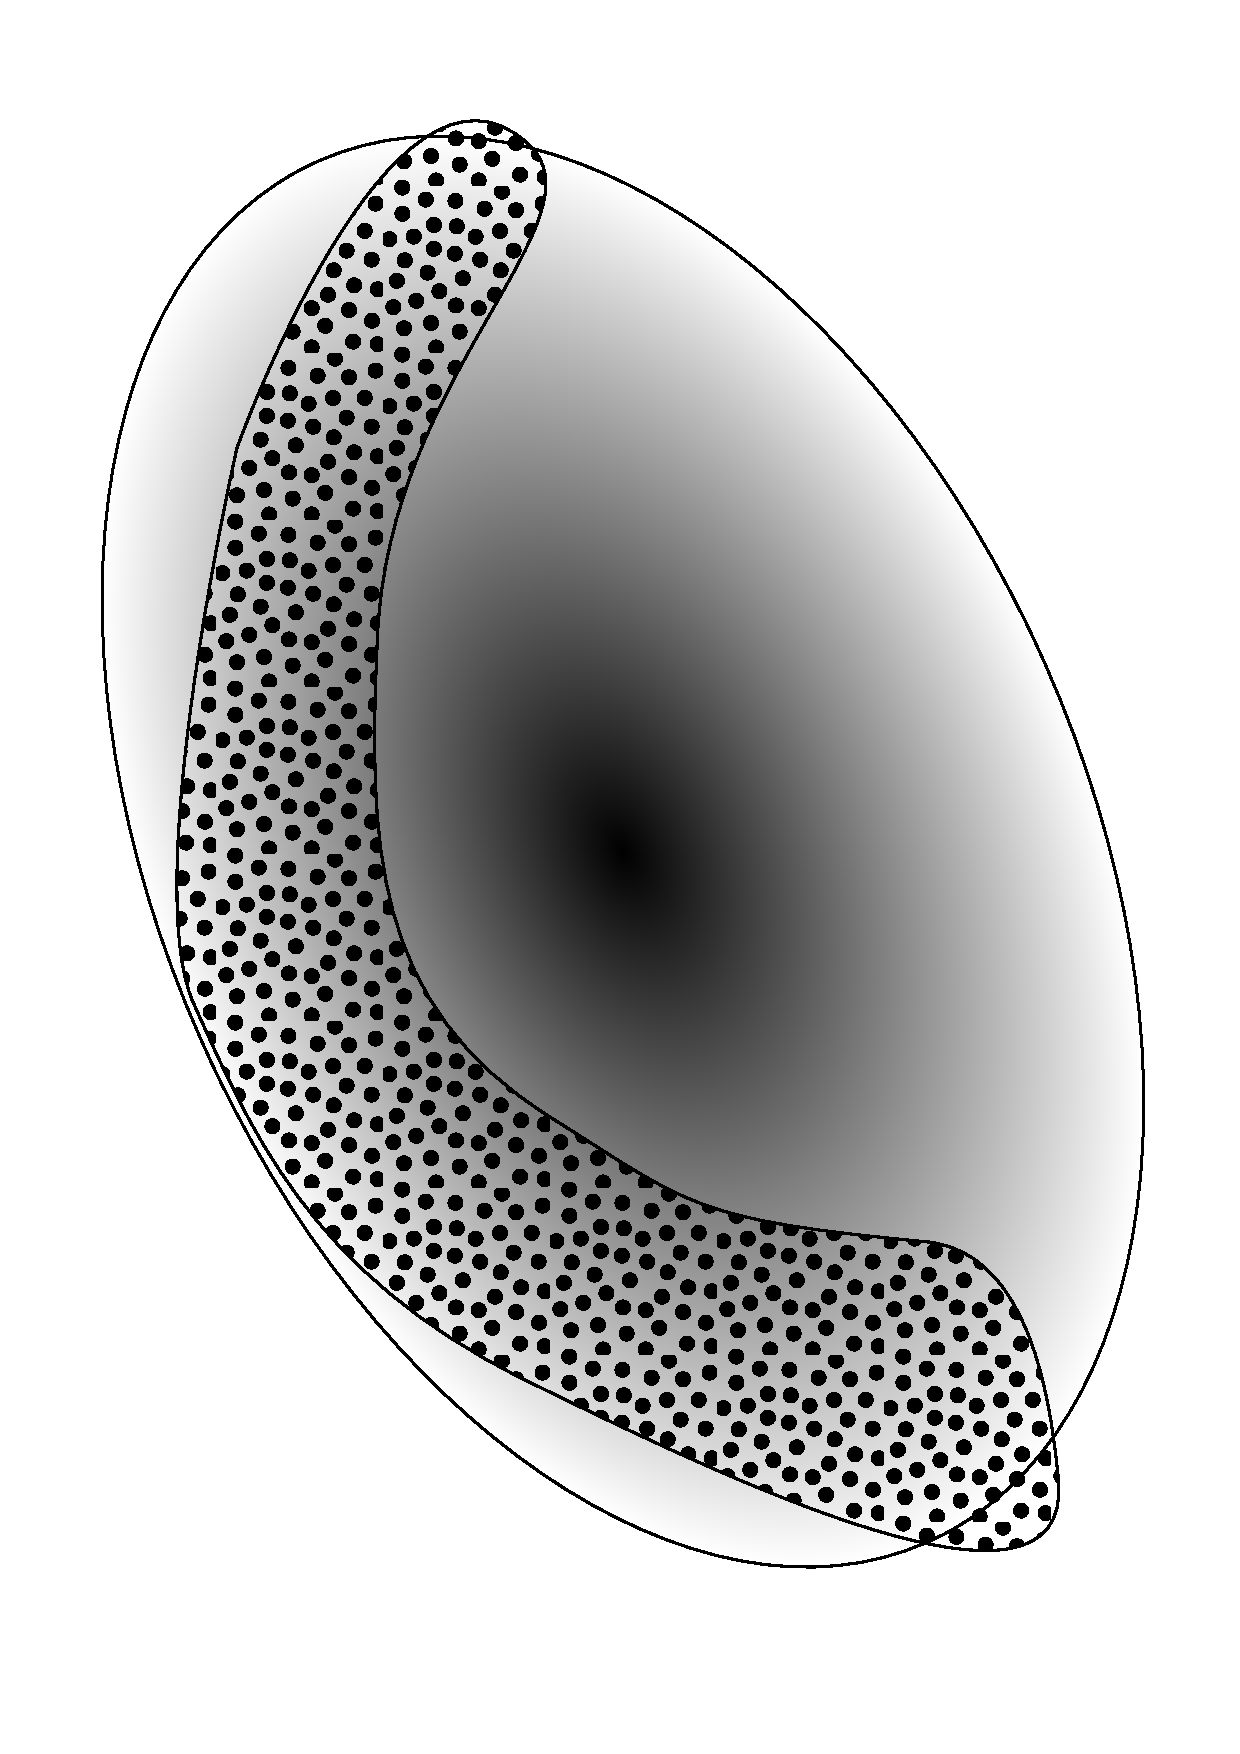
\includegraphics[scale=0.15]{clusterDensity/hardcluster1.pdf}
  }
  \fbox{
    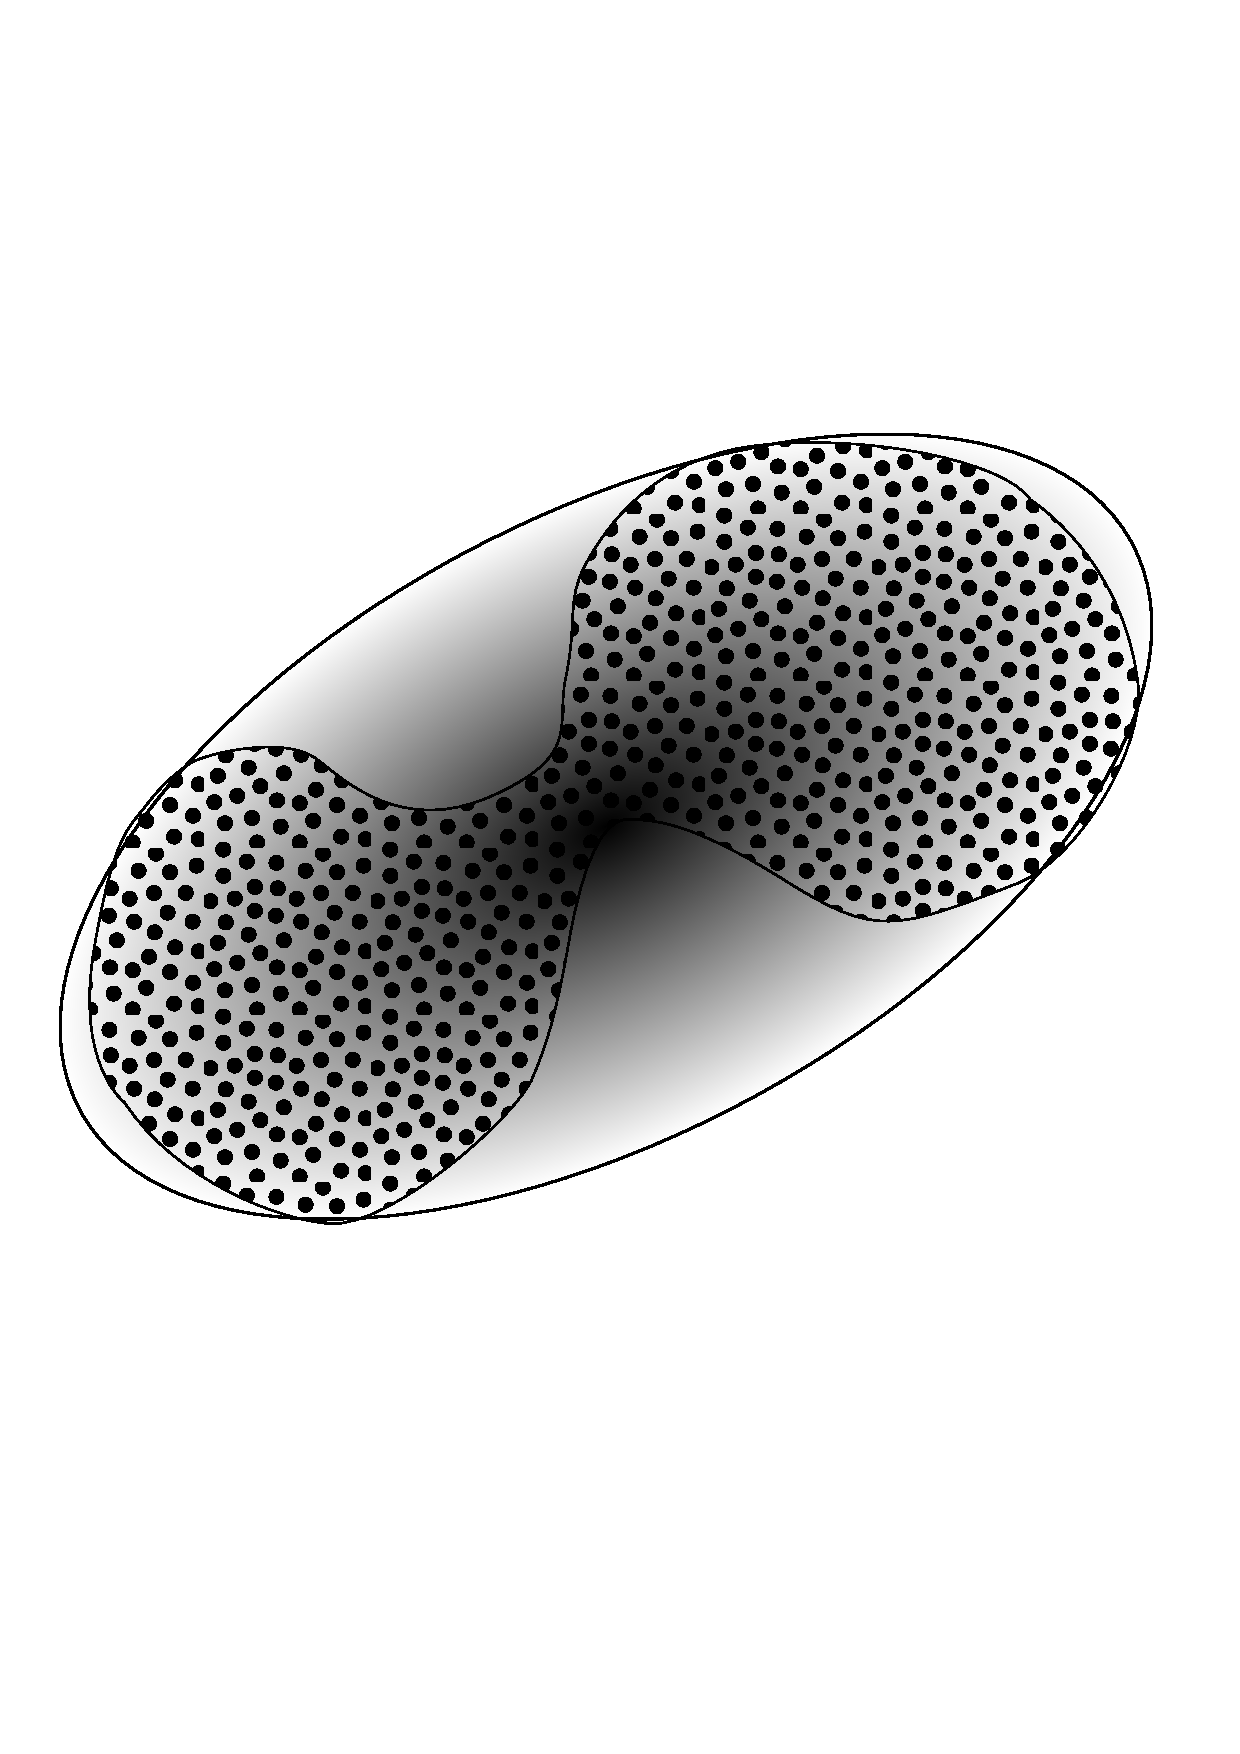
\includegraphics[scale=0.15]{clusterDensity/hardcluster2.pdf}
  }
  \caption{Example of two clusters returned by the clustering algorithm
  and corresponding Gaussian \textit{crunching functions} which degrade
  areas distant from clusters.}
  \label{fig:hardClusters1}
\end{figure}
 
 
To increase the accuracy of our algorithm
we use the following property of the OPTICS \textit{ordering}:
\begin{quotation}
\noindent
While creating the ordering, OPTICS constructs density-based clusters
with respect to different densities simultaneously. OPTICS ordering
actually contains the information about the intrinsic clustering structure of
the input data set (up to the generating distance $\epsilon$) 
(see \cite{optics}).
\end{quotation}

This might be shown for sample data (see Figure \ref{fig:opticsOrder1}) by using its
\textit{reachability plot}. Once we create OPTICS ordering
we may easily extract clusters with higher densities by decreasing
$\epsilon$ and choose clusters for which MSE (Mean--Square Error) 
between the actual fitness function and the crunching function in the 
areas of clusters is minimal.

The algorithm works as follows (see Algorithm \ref{alg:IFDA}): 
having the OPTICS ordering
of the population returned by the EA our method iteratively extracts 
clusters with higher densities by decreasing the \textit{neighborhood radius $\epsilon$} 
(see Figure \ref{fig:opticsOrder2}), and then by constructing crunching
function for extracted clusters and checking if the resulting crunching functions is more accurate than the best found in previous iterations (MSE comparison).

\begin{algorithm}
\caption{Improving fitness deterioration accuracy}
\label{alg:IFDA}
\begin{algorithmic}[1]
\STATE {$\epsilon'=\epsilon$}
\WHILE{$\epsilon' > treshold$}
	\STATE {$cs \leftarrow extractDBSCANClustering(\epsilon')$}
	\STATE {$crunchFs \leftarrow createCrunchingFunctions(cs)$}
	\STATE {$mse \leftarrow getMSE(crunchFs, currentFitness, cs)$}
	\IF{$mse < minMSE$}
		\STATE {$saveBestCrunching(mse, crunchFs)$}
	\ENDIF
	\STATE {$\epsilon' \leftarrow \epsilon' * 0.8$}
\ENDWHILE
\end{algorithmic}
\end{algorithm}

Algorithm \ref{alg:IFDA} effectively prevents the deterioration process
from destroying the fitness landscape in regions not yet explored by
the CSFD algorithm. 
Figure \ref{fig:hardClusters2} shows how the $\epsilon$
adjustment can improve the shape of the cluster extension
with respect to the initial one (see Figure \ref{fig:hardClusters1}).
To better understand how do we 
use OPTICS ordering to extract cluster of higher density see
Figures \ref{fig:opticsOrder1} and \ref{fig:opticsOrder2}.

\begin{figure}
  \centering
  \fbox{
    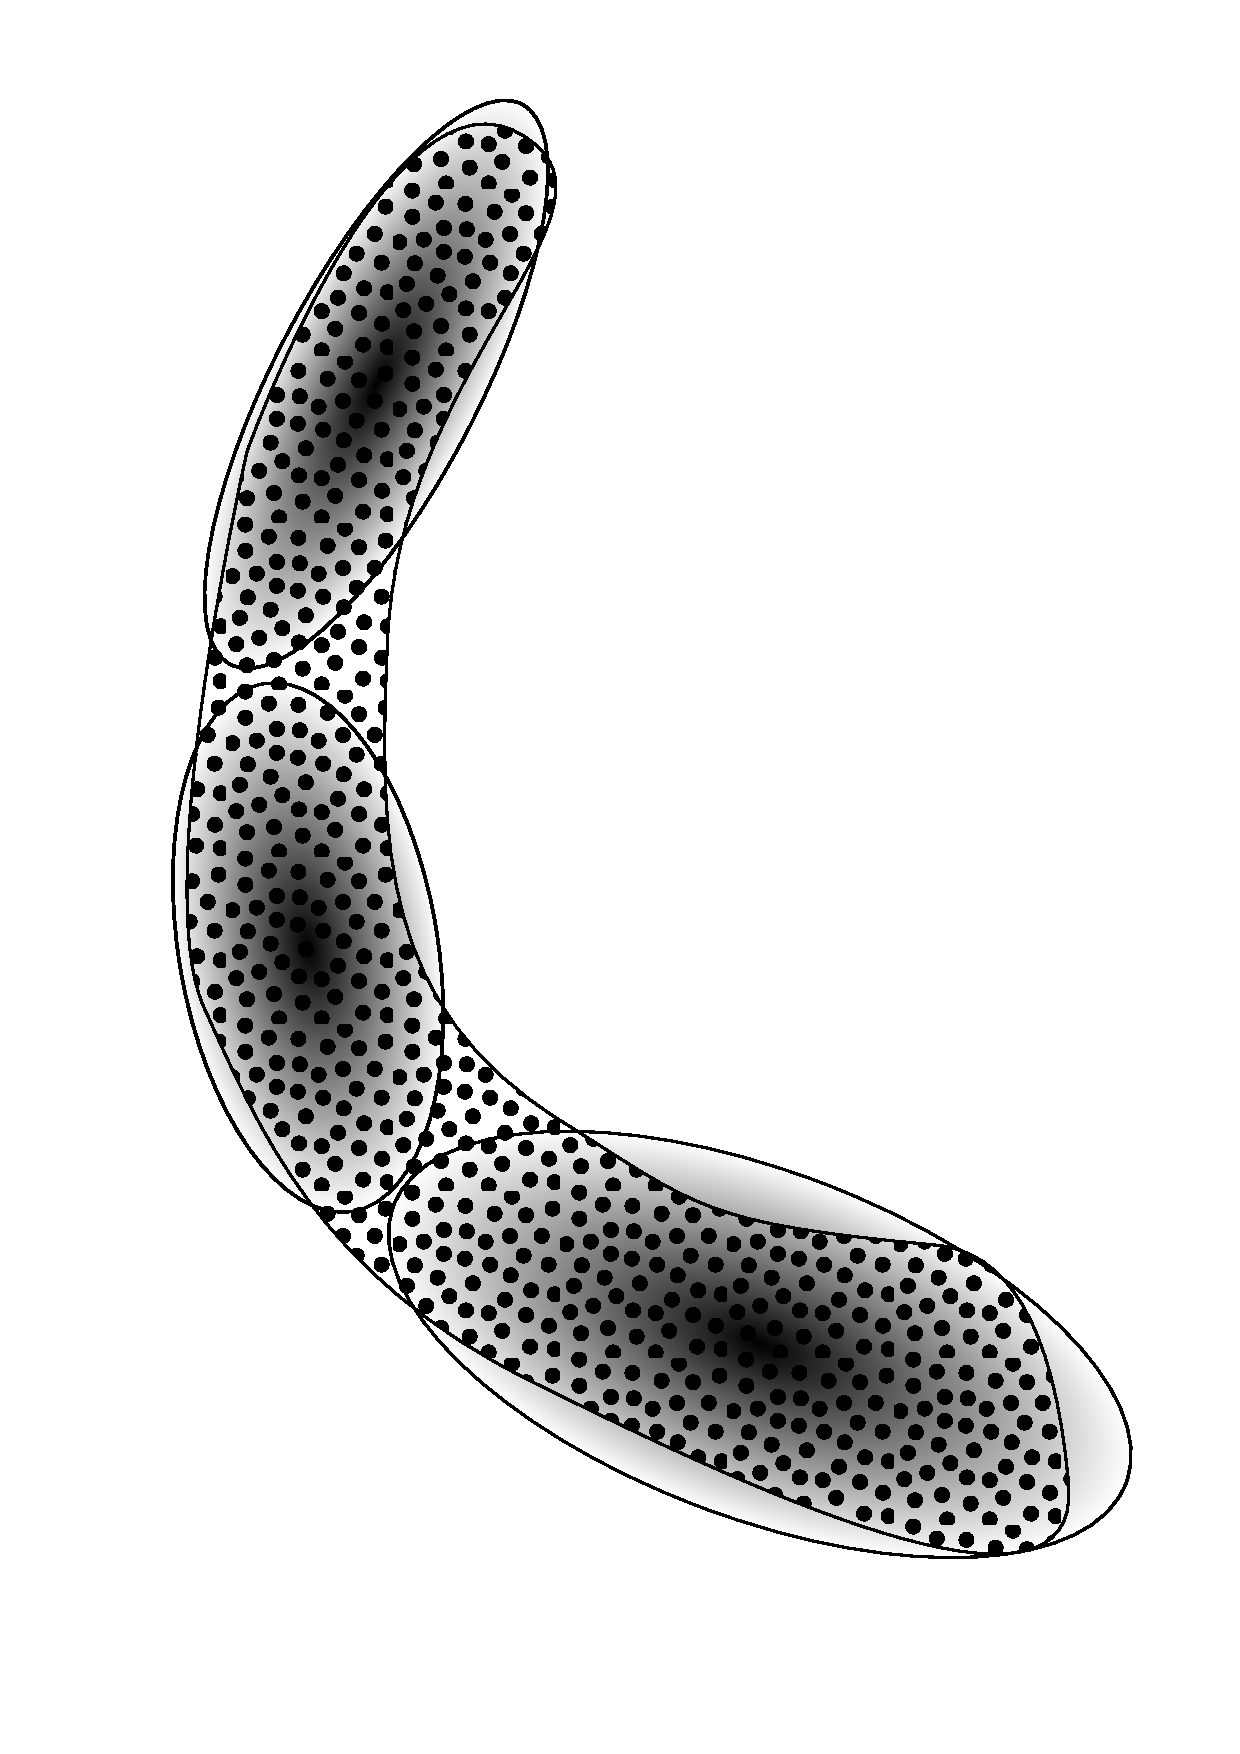
\includegraphics[scale=0.15]{clusterDensity/hardcluster12.pdf}
  }
  \fbox{
    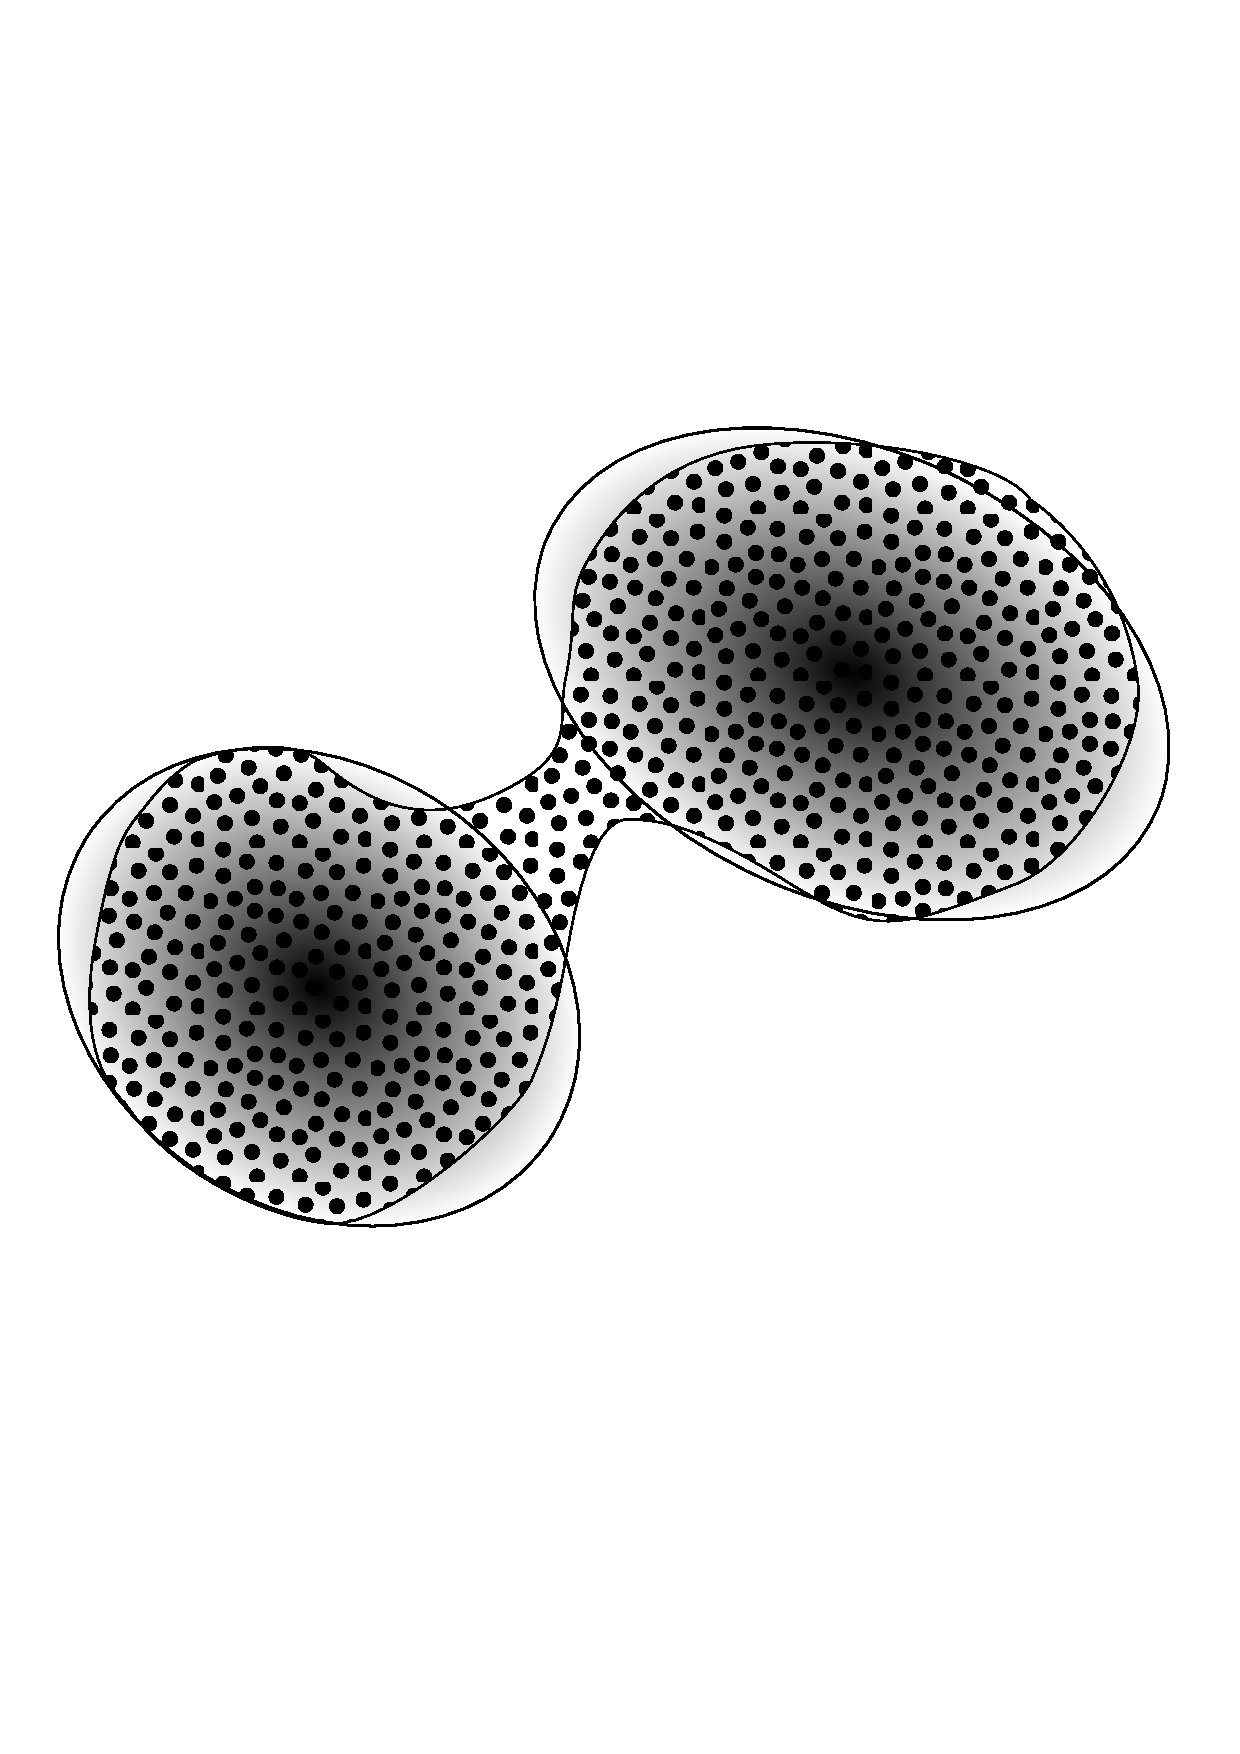
\includegraphics[scale=0.15]{clusterDensity/hardcluster22.pdf}
  }
  \caption{With \textit{OPTICS ordering} we may extract cluster of higher
  densities and minimize the impact of the fitness deterioration on regions
  outside the clusters (instead of creating one crunching function per cluster 
  like in figure \ref{fig:hardClusters1} we extract denser clusters from the
  \textit{ordering} and create crunching function which degrade only 
  the region occupied by the cluster)}
  \label{fig:hardClusters2}
\end{figure}



\begin{figure}
  \centering
  \fbox{
    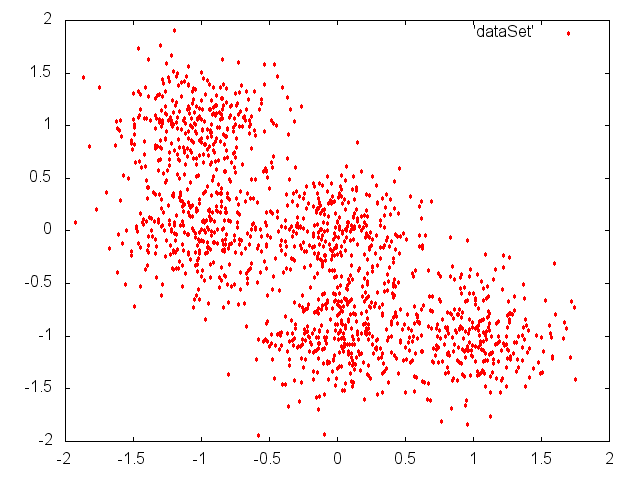
\includegraphics[scale=0.3]{clusterExtraction/extDataSet.png}
  }
  \fbox{
    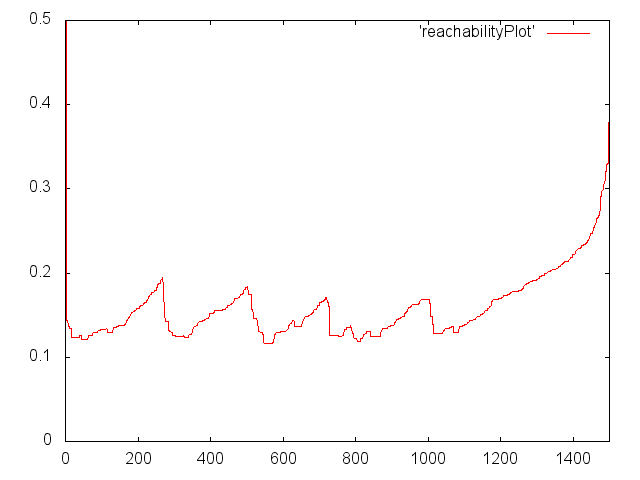
\includegraphics[scale=0.4]{clusterExtraction/reachabilityPlot.png}
  }
  \caption{Sample data set of 1500 points and the corresponding reachability plot
  of the ordered points (shows the reachability distance of each individual in the
  data set - horizontal axis corresponds to the individuals in the data set and
  the vertical axis shows the reachability distance of a given individual)
  OPITCS ordering parameters: $\epsilon=1.0$ $minPts=30$. 
  Cavities in the plot depict 5 clusters which might be extracted from the data
  set by the DBSCAN algorithm using proper value of $\epsilon'$ values}
  \label{fig:opticsOrder1}
\end{figure}

\begin{figure}
  \centering
  \fbox{
    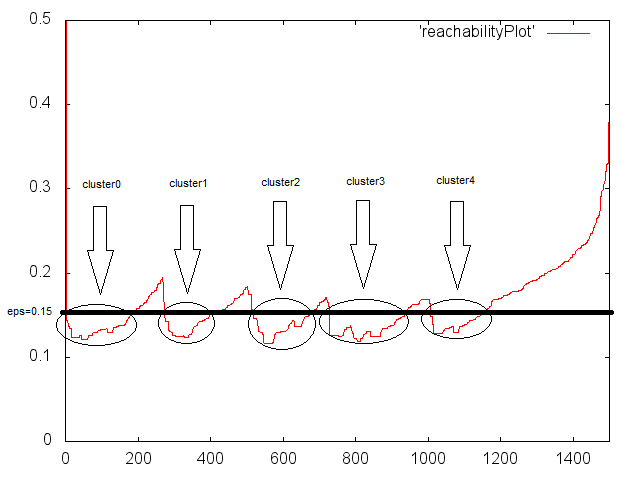
\includegraphics[scale=0.4]{clusterExtraction/reachabilityPlot1.png}
  }
  \fbox{
    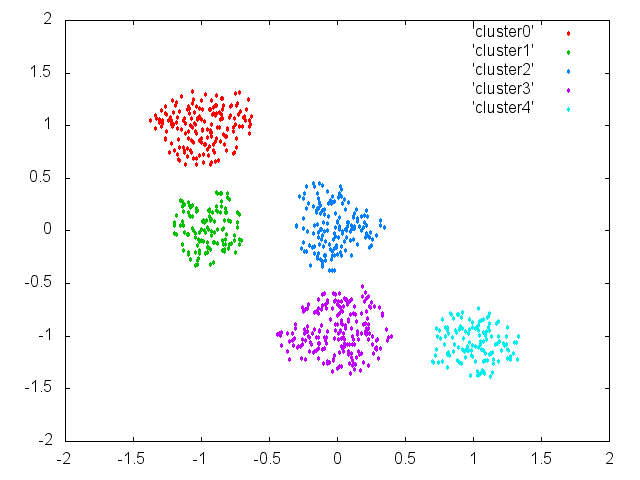
\includegraphics[scale=0.3]{clusterExtraction/extClusters.png}
  }
  \caption{Extraction of clusters from the data set presented in Figure
  \ref{fig:opticsOrder1} using DBSCAN algorithm with 
  $\epsilon'=0.15$. The value of $\epsilon'$ is marked on the first
  plot which shows reachability distances and the "cut off" clusters}
  \label{fig:opticsOrder2}
\end{figure}
 


\section{Basic Scheme}
\label{sec:BasScheme}

The basic version of our deterioration algorithm is as follows.
For each cluster $C$ generate a multi-dimensional Gaussian function
$g: V \rightarrow \mathbb{R}_+$
\begin{equation}
\label{eqn:GF}
g(x)= F_k(x_{max}) \,  exp \left(
 - \frac{1}{2}(x - \overline{m})^T \, \Sigma^{-1} \, (x - \overline{m})
\right)
\end{equation}
where $F_k$ is the fitness function in $k$-th iteration of the CSFD algorithm,
$x_{max}$ is the fittest individual from the cluster, the $\overline{m}$ is the
cluster's centroid (mean phenotype of invividuals belonging to $C$)
and $\Sigma$ is unbiased sample covariance matrix
estimated from the cluster population by the formula (\ref{eqn:Sigma})
(see e.g. \cite{SampleCovariance})
\begin{equation}
\label{eqn:Sigma}
\Sigma = \frac{1}{Card(C) - 1} \, \sum_{x \in C} 
(x - \overline{m}) \otimes (x - \overline{m})
\end{equation}
where $\otimes$ stands for the tensor product symbol. Please, notice, that
the sum in (\ref{eqn:Sigma}) is spanned over all individuals belonging
to the cluster $C$ i.e. the phenotype $x$ might be counted more than once,
if is repeatedly represented in $C$.


Fitness function in the $(k+1)$-th iteration is obtained from the equation
(\ref{eqn:fitDet}) by seting $\alpha_i \equiv 0, \, i = 1,\ldots,M_k$.



Big advantage of this algorithm are simplicity and speed.
However, this version may cause strong deformation of the
fitness landscape in areas which are distant from the already found clusters,
which is unacceptable. To overcome this issue we
developed so called \textit{weighted scheme} described 
in the next Section \ref{sec:WeightScheme}. 





\section{Weighted Scheme}
\label{sec:WeightScheme}

This type of fitness deterioration is more accurate and is likely to produce
more stable fitness that basic scheme, cause the latter may produce
sharp peaks in the fitness landscape, because of the very aggressive fitness degeneration.
Weighted Scheme is also more complex cause it generates
more computationally intensive fitness functions.

Initial steps are the same as in basic scheme, we create 
multi-dimensional Gaussian function for each cluster. 
What is different is how we compute the new (deteriorated) 
fitness is the following way
\begin{equation}
\label{eqn:WS1}
F_{k+1}(x) = F_k(x) + \sum_{i=1}^{M_k} \alpha_i(x) g_i(x),
\end{equation}
where the $\alpha$-coefficients are given by the following equations
\begin{equation}
\label{eqn:alpha1}
\alpha_1(x) \, +, \ldots, + \, \alpha_{M_k}(x) = 1,
\end{equation}
\begin{equation}
\label{eqn:alpha2}
\alpha_i(x) = \xi(x) \, \left( \frac{1}{r_i(x)} \right),
\end{equation}
\begin{equation}
\label{eqn:fractures}
\frac{1}{\xi(x)} = \frac{1}{r_1(x)} \, +, \ldots, + \, \frac{1}{r_{M_k}(x)},
\end{equation}
where $r_i(x) = \left\| x - \overline{m}_i \right\|$ is the distance between $x$ 
and the $C_i$ centeroid $\overline{m}_i$ (see Figure \ref{fig:weightedScheme}). 
So in order to compute fitness for a 
given individual $x$ (more correctly for $ph(x)$) 
we have firstly compute distances $r_i(x)$. 
Then we compute $\xi(x)$ from the equation (\ref{eqn:fractures}), next the
$\alpha$-coefficients from the system (\ref{eqn:alpha1}),(\ref{eqn:alpha2})
and finally the fitness value from (\ref{eqn:WS1}).
$\alpha$-coefficients are computed separately for each new individual 
and this is why this method is more costly than the previous one.
\begin{figure}
  \centering
  \fbox{
    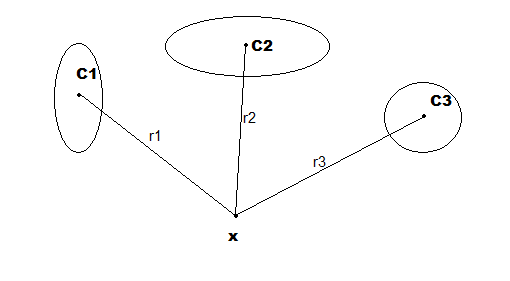
\includegraphics[scale=0.4]{AdaptiveScheme.png}
  }
  \caption{The coefficient $\alpha_i$ is inversely proportional to the 
  distance from the center of cluster $C_i$ to the $x$. $\alpha_i$ may
  be seen as the impact $C_i$ has on $x$}
  \label{fig:weightedScheme}
\end{figure}
From the equations (\ref{eqn:WS1})-(\ref{eqn:fractures}) 
it is clear that regions of domain
which are distant from clusters found in previous iterations of the algorithm
are very little affected by the crunching functions which is a big advantage
over the basic scheme. 
However, experiments shows that the basic
scheme yields very good results and is preferable over the weighted
scheme due to the lower computational cost of the former.



\section{Crunching Function Adjustment}
\label{sec:CrumchAdj}


Because of the fast convergence of populations
generated by the GA algorithm to the local solutions 
and the features of the Algorithm \ref{alg:IFDA} used
to increase accuracy of the deterioration process, %(see Section \ref{sec:OPTICS}),
clusters sometimes become very dense in areas close to the local minimizers. 
Gaussians created for such
clusters does not approximate a basin of attraction well, speaking informally:
Gaussian functions created for such clusters consist of high and thin peaks
which deteriorate only the area inside the cluster, 
only the narrow basin of attraction
in which the cluster resides.
To overcome this issue we developed so called \textit{Crunching Function
Adjustment} (CFA) algorithm described below.


We use sample covariance matrix as an estimator (see \cite{SampleCovariance}), which
is extremely sensitive to outliers. However we may take this property as our
advantage and incorporate it CFA algorithm. 
Having given a cluster of points the CFA algorithms works as follows:

\begin{itemize}

  \item We estimate the covariance matrix $\Sigma$ 
  and then compute its $N$ eigenvectors
  ($N = dim(V)$ is the dimension of the problem space). 
  They are ortogonal one to each other
  and define the orientation of the Gaussian "bell"
  
  \item for each eigenvector $v_i$ we generate two points 
  $\underline{p_i}, \overline{p_i}$ called \textit{leading marks}
  \begin{eqnarray}
  \label{eqn:outliners}
  \overline{p_i} = \overline{m} + \sqrt{\lambda_i} \, v_i \nonumber\\
  \underline{p_i} = \overline{m} - \sqrt{\lambda_i}\, v_i
  \end{eqnarray} 
  where $\overline{m} \in V$ is the cluster's centroid and $\lambda_i$ is
  an eigenvalue of the eigenvector $v_i$.
  
  \item Then we add these $2 N$ generated leading marks to the initial
  multiset which constitute a cluster, and compute new covariance matrix.
  
  \item Because the sample covariance matrix is very sensitive to leading marks,
  the resulting covariance matrix produces a Gaussian function whose "bell
  hypersurface" is more stretched in directions of eigenvectors.
  
  \end{itemize}
  
Please notice, that the improvement introduced above is purely heuristic,
having no precise mathematical motivation. It was designed only
for deterioration performed by Gauss functions and positively verified for
2D benchmarks (see Section \ref{sec:testFun}) so its usefulness 
in other cases in unknown.

\subsection{CFA Results}

The figures below shows the result of our CSFD algorithm with CFA for two
simple functions from $f:\mathbb{R}^2 \rightarrow \mathbb{R}$, specifically:
\begin{itemize}
  \item $f(X) = 2e^{-(x^2 + y^2)}$, where $X \in \mathbb{R}^2$
  \item $f(X) = e^{-(x^2 + y^2)}+1.4e^{-((x-1.7)^2 + (y-1.7)^2)}$, where $X \in
  \mathbb{R}^2$
\end{itemize}

\begin{table}[ht]
    \caption{The results of basic deterioration scheme applied to functions 
    $f(X) = 2e^{-(x^2 +y^2)}$ (up-left and down-left) and $f(X) = e^{-(x^2 +
    y^2)}+1.4e^{-((x-1.7)^2 + (y-1.7)^2)}$ (up-right and down-right) with the
    populations generated with normal distribution around the solutions. For
    the fist function we may see that the 
  	overall landscape decreases only by $30\%$ (down-left), while using
  	CFA gives us $85\%$ of decline (up-left). For the second function we
  	see $25\%$ of deterioration (down-right), while CFA gives us $78\%$
  	(up-right)}
    \centering
    \begin{tabular}{cc}
    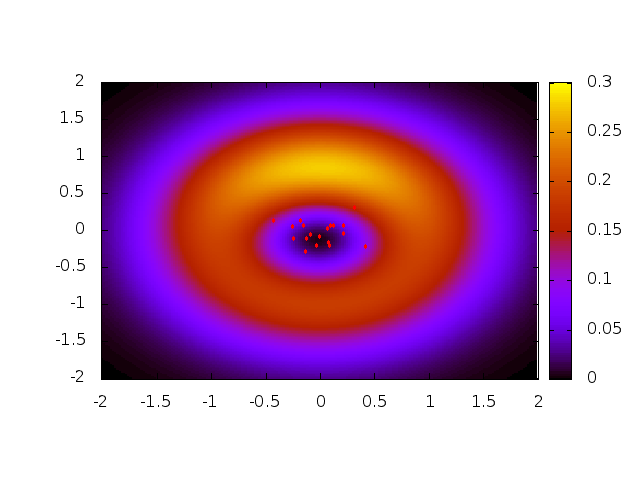
\includegraphics[scale=0.3]{CMA/result1_CMA.png} &
    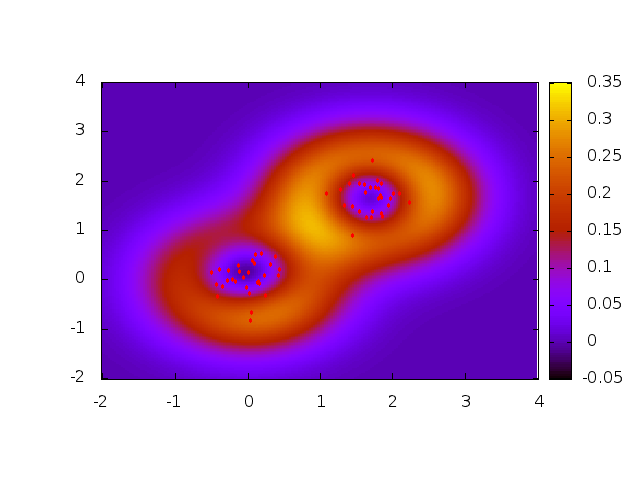
\includegraphics[scale=0.3]{CMA/result2_CMA.png} \\
    \newline
    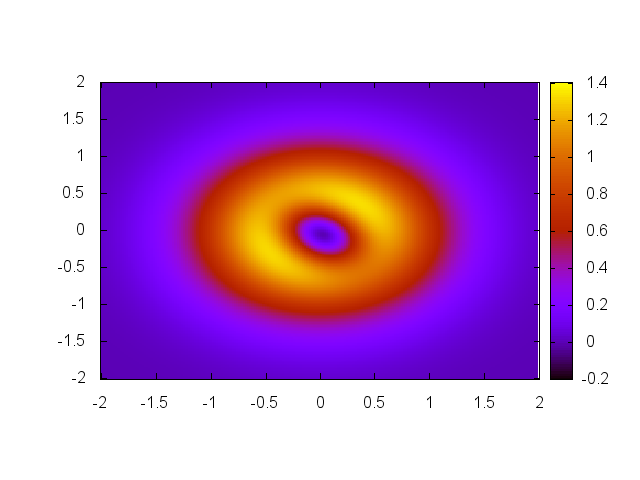
\includegraphics[scale=0.3]{CMA/result1_noCMA.png} &
    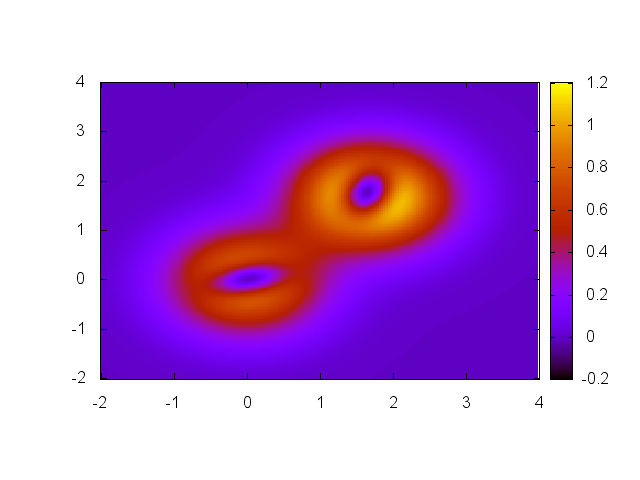
\includegraphics[scale=0.3]{CMA/result2_noCMA.png} \\
    \end{tabular}
    \label{tab:cfa}
\end{table}%

Table \ref{tab:cfa} shows how much the algorithm benefit
from using the CFA algorithm.



\chapter{Tested Algorithms}
\label{TestedAlgorithms}


\section{HGS}
why HGS is well suited to our algorithm (suitable for clustering, fast
convergence in leaves)

\section{Tests}

\subsection{Benchmark functions}
uni, bi and multimodal functions

\subsection{Accuracy measures}
how many optimas have been found,
diagrams

\subsection{Efficiency measures}








\chapter{Implementation}
\label{ch:Implementation}
To verify our algorithm we have created a simple, global optimization framework
which enabled us to execute and test all of the algorithms described throughout
this article.

We decided to use Java as a programming language and runtime
environment for this project. 

Using the framework we can find optima of real, mulimodal, multidimensional and
continuous functions. We just need to provide the framework with the concrete
fitness function implementation, and by specifying the problem domain.

The framework principle is to separate the interfaces from implementation.
Our API provides interfaces for evolutionary algorithms, fitness assignment
and fitness deterioration, genetic operators like selection and reproduction,
phenotype, clustering algorithms and many more. This makes it compact,
extensible and easy to introduce new implementations.
For the detailed description of the classes and interfaces see section
\ref{sec:impl}.

\section{Architecture}
\label{sec:architecture}

The project consists of six main packages, which communicates with the
others through clearly specified interfaces and together constitute a
complete, lightweight framework for testing and execution of the global 
optimization algorithms especially the evolutionary algorithms.
\begin{itemize}
  \item \textit{Algorithm module} - central module of the framework. Contains
  implementation of the \textit{Cluster Supported Fitness Deterioration}
  algorithm described in chapter \ref{ch:csfdAlgorithm}. The main class in the module
  \textit{ki.edu.agh.algorithm.SequentialNichingWithOpticsClustering} is
  responsible for creation of the Spring context and execution of the algorithm. 
  \item \textit{Clustering module} - contains interfaces for clustering
  algorithms and implementation of OPTICS.
  \item \textit{Fitness deterioration module} - contains implementation of
  \textit{FitnessDeterioration} interface. Most important are:
  \textit{ki.edu.agh.deterioration.SimpleGaussianFitnessDeterioration} and 
  \textit{ki.edu.agh.deterioration.WeightedGaussianFitnessDeterioration}.
  \item \textit{Evolutionary Algorithms module} - contains all the necessary
  interfaces for EA, selection and reproduction operators, individuals and
  phenotypes. Implementations of SGA and Evolution Strategy. 
  \item \textit{Printing Modul} - used to print populations and fitness
  landscape during the program execution
  \item \textit{Statistics Utils} - based on JAMA. This package
  contains many useful statistical functions, e.g. CFA algorithm, covariance
  matrix estimation, multidimensional Gaussian function, fitness deterioration
  untilities.
\end{itemize}

\section{Implementation in Java}
\label{sec:impl}

The framework was written to be elegant and extensible. The system's 
modules are loosely coupled and each of its components has little knowledge of
the definitions of the others (see previous section). This
allows for extensibility in further design. To implement the system we used Spring
as an application framework, Maven for project
management and build automation, JUnit and Mockito
for testing and Git as revision control system. 
The source code, configuration files and sample results may be found at 
GitHub: https://github.com/wolny/Fitness-Deterioration

\subsection{Technologies}
\begin{itemize}
  \item Spring - application framework
  \item Maven - project management and build automation
  \item Mockito - testing framework 
  \item JAMA - linear algebra package
\end{itemize}


\chapter{Conclusions}
\label{Conclusions}

\section{Summary}
The aim of my Master Thesis was to find an effective fitness deterioration
algorithm as defined in chapter 4, which minimizes the chance of multiple
exploration of the same solution during the course of the \textit{Sequential
niching} algorithm. Taking into account the results of tests described in
chapter 5 we may come to the conclusion that the goal was reached. However,
tests was performed only for simple
multimodal problems in which the obtained clusters were convex and provides 
a lot of information about underlying basins of attraction. Applying the
algorithm for more demanding functions should be the next step in the further
development of the algorithm.  

The assumption that distribution of individuals inside a cluster provides
information about its shape oversimplifies the real nature of the evolutionary
algorithms, where the population distribution inside basins of attraction is 
very hard to predict and depends on many factors, including recombination versus
mutation rate, selection algorithm, definition of genetic operators such as
mutation and crossover. We can expect satisfactory results when
choosing proportionate selection and genetic operators which are based on normal
distribution. \textit{Fitness Proportionate Selection} usually causes faster
convergence to local solutions and normal distribution based reproduction operators tends 
to produce populations with useful information about fitness landscape.

Choosing weighted crunching functions for \textit{Fitness deterioration}
(as described in section 4.3) is always more accurate than the
\textit{Basic scheme} described in section 4.2. 
You can sacrifice accuracy for speed when fitness function
evaluation is very costly by using the \textit{Basic scheme}.

The most valuable outcomes of this work are:
\begin{itemize}
  \item definition and implementation of a hybrid metaheuristic called \textit{Sequential
  niching} which may be used for solving multimodal optimization problems.
  \item applying clustering algorithms as a reasonable stop criterion for
  real-valued evolutionary algorithms
  \item using properties of \textit{OPTICS ordering} \cite{optics} to improve
  the deterioration process
  \item definition and implementation of two variants of the fitness
  deterioration algorithm which might be used in different scenarios depending
  on the expected speed and accuracy of the global optimization
  \item definition and implementation of the \textit{Covariance Matrix
  Adaptation} algorithm which improves the efficiency of the fitness
  deterioration
  \item creation of an extensible, lightweight framework which implements all of
  the algorithms and ideas presented in this work and which can be used for
  further research
\end{itemize}


\section{Future Research}

This work focuses mainly on the \textit{Fitness Deterioration} algorithm and
shows the result of Basic and Weighted variants of the algorithm applied to
simple multimodal functions (see chapter 4). Given the \textit{Sequential
niching} algorithm described at the beginning of this paper (chapter 2), the main
direction of the future research should be to test this algorithm using many 
different evolutionary algorithms and evolution strategy.
The most promising algorithm to choose would be \textit{Hierarchical Genetic
Strategy} (HGS) \cite{hgs}.

The Hierarchical Genetic Strategy (HGS) performs efficient concurrent
search in the optimization landscape by many small populations. The creation of
these populations is governed by dependent genetic processes with low complexity
\cite{hgs}. HGS is an example of parallel genetic algorithms and it performs
very well especially in case of problems with many local extrema.
Taking into account the fact that HGS is likely to find many solutions in a
single run of the algorithm and that the hierarchy of populations generated
by the algorithm are rapidly convergent it would be very efficient 
from the standpoint of the deterioration process.

There are many aspects of the implementation of \textit{Sequential
niching} algorithm, described in chapter 6, which can be improved as well. 
The framework uses very simple concurrency model which may be further
developed to improve the overall performance of the algorithm.
The most costly stages of the algorithm include: fitness function computations
during EA algorithm and creation of \textit{OPTICS ordering} \cite{optics}.
The former problem might be solved by introducing some of the known
parallel genetic algorithms and the latter might be tackled by proper
domain decomposition. If we want to introduce a highly concurrent EA model
again it would be best to use HGS because of its natural concurrent character.


\appendix

\chapter{Installation and Program Results}
\label{ch:instResult}

\section{Installation and Execution Instructions}
\label{sec:installation}

\begin{itemize}
  \item Configuration files: \textit{application-context.xml} - here you
  specify used algorithms, problem domain, fitness function and other aspects
  of the system (see sample configuration in appendix B); some of the most
  important properties are taken from \textit{algorithm.properties} file
  using property placeholders 
  \item To build the project invoke: \textit{mvn clean install}. 
  \item Program execution: \textit{mvn exec:java} By default the main class of
  the project is:
  \textit{ki.edu.agh.algorithm.SequentialDeteriorationEAWithOpticsClustering}
  (see \textit{pom.xml} for more details)
\end{itemize}

\section{Program Results}
\label{sec:results}

Program saves the results in 'diagrams' catalog:
\begin{itemize}
 \item cluster's members are stored in files of the name 'clusterN', where N is
 the number of cluster 
 \item populations for each run are stored in files
 'populationN', where N is the number of EA run 
 \item fitness landscape is stored in file 'originalFitnessLand'
 \item reachablity plot for OPTICS algorithm is stored in ''reachabilityPlot'
 \item fitness landscape after each run is stored in 'fintessLand\_iterN' where
 N is the number of EA run
\end{itemize}


\chapter{Installation and Configuration}
\label{Installation and Configuration}

\section{Installation and Execution Instructions}

\begin{itemize}
  \item Configuration file: \textit{application-context.xml} - here you specify
  used algorithms, problem domain, fitness function and other aspects
  of the system (see sample configuration below)
  \item To build the project invoke: \textit{mvn clean install}. 
  \item Program execution: \textit{mvn exec:java} By default the main class of
  the project is:
  \textit{ki.edu.agh.algorithm.SequentialDeteriorationEAWithOpticsClustering}
  (see \textit{pom.xml} for more details)
\end{itemize}

\section{Program Results}
Program saves the results in 'diagrams' catalog:
\begin{itemize}
 \item cluster's members are stored in files of the name 'clusterN', where N is
 the number of cluster 
 \item populations for each run are stored in files
 'populationN', where N is the number of EA run 
 \item fitness landscape is stored in file 'originalFitnessLand'
 \item reachablity plot for OPTICS algorithm is stored in ''reachabilityPlot'
 \item fitness landscape after each run is stored in 'fintessLand\_iterN' where
 N is the number of EA run
\end{itemize}


\section{Sample Spring configuration}
\lstinputlisting{test-context.xml}


\bibliographystyle{alpha}
\bibliography{fitness-deterioration}

\end{document}
